% !TEX encoding = UTF-8
% !TEX TS-program = pdflatex
% !TEX root = ../tesi.tex
% !TeX spellcheck = it_IT


%**************************************************************
\chapter{Progettazione}
\label{cap:progettazione}
%**************************************************************

Una volta acquisite delle conoscenze teoriche che mi permettessero di affrontare l'argomento mi sono reso conto che avrei avuto bisogno di un algoritmo che si prendesse carico di svariati passi:
\begin{enumerate}
	\item generare un \textit{dataset} compatibile col linguaggio delle API di \grayname{Tensorflow}\cite{prod:tensorflow};
	\item usare i pesi di una rete già allenata e che fosse compatibile con i miei scopi sfruttando il \textit{transfer learning} per creare un grafo personalizzato con cui fare inferenza poi;
	\item elaborare un file PDF su cui fare inferenza, sfruttando il grafo di cui sopra, per generare del testo puro e dei dati tabellari su CSV.
\end{enumerate}
A questo scopo mi sono presto convinto di dover sviluppare due progetti ben distinti: \grayname{TableTrainNet}\cite{prod:TableTrainNet} e \grayname{IntelligentOCR}\cite{prod:IntelligentOCR}. Il primo si sarebbe occupato di elaborare il \textit{dataset} col quale avrei allenato la mia rete neurale, il secondo invece avrebbe gestito una \textit{pipeline} che si sarebbe occupata della conversione da PDF a testo e csv.

%**************************************************************
\section{Tecnologie e strumenti utilizzati}
\label{sec:tecnologie-strumenti}
    \subsection{Codice e versionamento}
    Per entrambi i progetti è stato utilizzato il linguaggio di programmazione Python\cite{prod:python} versione 3. Inoltre, come raccomandato in azienda, è stato fatto l'utilizzo di \grayname{PyCharm}\cite{prod:PyCharm}, un IDE per Python dell'azienda Jetbrains\textsuperscript{\textcopyright{}} che, oltre ad offrire un assistente "intelligente" per la scrittura di codice e \textit{safe refactoring}, include anche degli strumenti di sviluppo quali \textit{debugging} e \textit{deploying} su GitHub\cite{site:github}. Si è fatto uso di quest'ultimo strumento per il versionamento del codice, che può essere trovato alle \textit{repositories} citate in bibliografia.
    \medskip
    \\Da notare, infine, che tutto il codice è regolabile da comodi files contenenti solamente "costanti". Queste "costanti", che poi non sono altro che le variabili che l'utente può e deve personalizzare per far funzionare il prodotto sulla propria macchina, si occupano di gestire tutto il funzionamento del prodotto, gestendo gli input, i modificatori e gli output.

    \subsection{Allenamento di reti neurali e inferenza}
    Per tutta la parte di intelligenza artificiale mi sono affidato al framework \grayname{Tensorflow}\cite{prod:tensorflow}. \grayname{Tensorflow} è una libreria \textit{open source} per computazione numerica ad alte prestazioni. Mi sono reso conto quasi subito che non avrei avuto il tempo di costruire una rete personalizzata per mancanza di tempo. Tra i prodotti "pre-confezionati" e che mi avrebbero permesso poi una certa personalizzazione senza dover avere troppo a che fare con del codice "a basso livello" è stata per l'appunto l'API di \textit{object detection}\cite{prod:tensorflow_o_d_api}. Questa libreria permette, utilizzando il \textit{core} di Tensorflow, di allenare e valutare reti neurali a partire da file di configurazione personalizzati. Alcuni parametri salienti che sono modificabili sono, per esempio:
    \begin{itemize}
    	\item il \gls{learning rate} e le varianti ad esso associate;
    	\item la \gls{batch size};
    	\item la tipologia di \textit{optimizer};
    	\item alcune opzioni di \gls{data augmentation};
    	\item i \textit{checkpoint} di partenza, da quali prendere i pesi di altre reti neurali per approfittare del \textit{transfer learning}.
    \end{itemize}
    Questi sono solo alcuni dei parametri messi a disposizione e dei quali parlerò più profusamente durante la descrizione del progetto \grayname{TableTrainNet}. Da notare infine che assieme a questa libreria sono stati messi a disposizione anche dei pesi di partenza, ovvero le reti già pre-allenate che poi ho utilizzato nel corso del mio progetto. Inoltre \grayname{Tensorflow} mette nativamente a disposizione uno strumento di controllo automatico dell'andamento dell'apprendimento della rete chiamato \grayname{Tensorboard}.
    \medskip
    \\Per quanto riguarda l'inferenza, \grayname{Tensorflow} non si è dimostrato il framework dal linguaggio più semplice da utilizzare - \grayname{Keras}\cite{prod:keras} utilizza una sintassi molto meno complessa -. Tuttavia, la documentazione online è molto buona e l'utilizzo del framework per ottenere delle \textit{boxes} a partire da immagini è standard e ben comprovato.

    \subsection{\textit{Editing} di immagini}
    Il progetto si è principalmente basato sulle immagini: avevo bisogno di strumenti efficaci che mi permettessero di perdere il meno tempo possibile nelle impostazioni, per poterlo poi impiegare nella valutazione dei risultati.
        \subsubsection*{Pillow}
        Ho trovato in \grayname{Pillow}\cite{prod:pillow} veramente rapido nell'utilizzo per ottenere immagini dal disco o da \textit{arrays}, farne dei ritagli, convertirle in scala di grigi e poi salvarle sul disco. 
        \subsubsection*{OpenCV}
        Per quanto riguarda invece modificazioni un po' più complesse ho utilizzato invece \grayname{OpenCV}\cite{prod:cv2}, che lavora su immagini sotto forma di array ed è più orientata al \textit{machine learning} e al \textit{computer vision}. 
        \subsubsection*{Alyn con Scikit-image}
        Ho inoltre utilizzato uno strumento di raddrizzamento automatico delle immagini, \grayname{Alyn}\cite{prod:alyn}, modificando un progetto che avevo trovato valido, correggendolo e adattandolo alle mie esigenze. Questo progetto fa uso di \grayname{Scikit-image}\cite{prod:scikit-image}.

    \subsection{Estrazione di informazioni}
        \subsubsection*{Da PDF ad immagini}
        \grayname{pdftoppm}\cite{prod:pdftoppm} si è dimostrato il miglior strumento per estrarre immagini a partire da PDF. Inizialmente avevo usato un \textit{wrapper} attorno a \grayname{ImageMagik}\cite{prod:imagemagik}, ma con PDF di grandi dimensioni il programma non riusciva a gestire i files temporanei, causando un intasamento del computer in cui era eseguito.
        \subsubsection*{Da PDF a tabelle}
        \grayname{Tabula}\cite{prod:tabula} è un'applicativo Java che si occupa di interpretare un foglio PDF per estrarre tutte le possibili tabelle ed esportarle in un CSV, utilizzando \grayname{pandas}\cite{prod:pandas}.
        \subsubsection*{Da immagini a testo}
        Per estrarre il testo a partire da immagini ho usato \grayname{Tesseract}\cite{prod:tesseract}. Questo è un motore OCR per il riconoscimento di caratteri all'interno di un'immagine, che è stato sviluppato inizialmente ai laboratori in Bristol di Hewlett-Packard. \'E stato reso pubblico nel 2005 e poi sviluppato da Google. Ho usato la versione 4, attualmente in sviluppo attivo, che fa uso di una rete neurale \glslink{lstm}{LSTM} per migliorare l'individuazione dei caratteri. Non mi sono occupato di allenare questa rete, ma ho usato l'allenamento offerto direttamente da Google.
\newpage
\section{TableTrainNet: creare il \textit{dataset}}
Questo progetto è stato sviluppato per creare una rete neurale che riconosca tabelle all'interno di documenti. Il prodotto di questo progetto serve poi ad \grayname{IntelligentOCR} per funzionare.
    \subsection{\textit{Overview} generale}
    Il progetto usa una delle reti neurali offerte\cite{prod:tensorflow-model-zoo} da \grayname{Tensorflow} per analizzare un \textit{dataset} contenente immagini con tabelle. In più è stato personalizzato un file di configurazione per l'allenamento e valutazione per utilizzare l'API di \textit{object detection}\cite{prod:tensorflow_o_d_api}.
    \subsection{Il \textit{dataset} iniziale}
    La prima difficoltà di creare un buon \textit{dataset}, inutile a dirsi, è trovare una buona base. Sebbene siano molto comuni insiemi di immagini relative ad oggetti generici, sono altresì rari quelli relativi agli oggetti che si possono trovare nei documenti. \'E stato quindi inizialmente complesso trovare delle immagini con documenti già etichettati, senza dovermeli creare da solo.
    Fortunatamente sono entrato in contatto con una competizione online di \glslink{pod}{POD}\cite{site:ICDAR-2017-POD} organizzata dall'Università di Pechino, Istituto di \textit{Computer Science and Technology}\cite{site:comp-sci-peking}. Il \textit{dataset} è formato da 2000 documenti in inglese selezionati da 1500 articoli scientifici di \textit{CiteSeerX}\cite{site:cite-seer-x}, contenenti sia tabelle che formule e grafici. Mostra poi una buona varietà sia per quanto riguarda il \textit{layout} della pagina, sia per lo stile degli oggetti, includendo testo a singola e doppia colonna.
    \begin{figure}[H] 
        \centering
        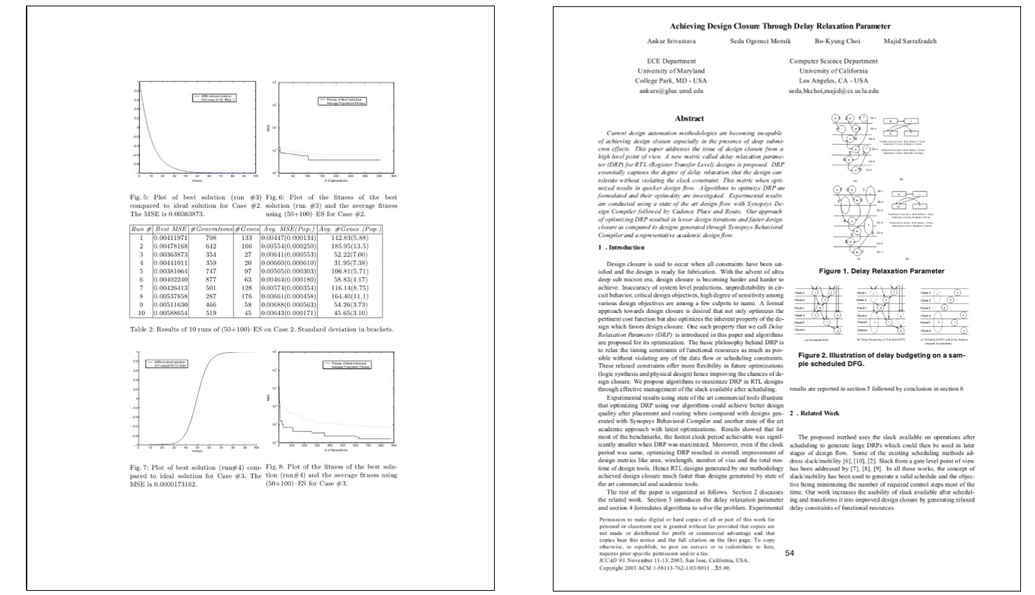
\includegraphics[width=1\columnwidth]{esempi_immagini_dataset_1} 
        \caption{Esempio di immagini presenti nel dataset}
        \label{img:example_dataset_images}
    \end{figure} 
    Per quanto riguarda il mio progetto ho preso in considerazione solamente le tabelle, ignorando le altre informazioni che si possono trovare. Dovendo infatti orientare la mia rete neurale ad analizzare polizze assicurative, ho preferito evitare di inserire elementi di disturbo - ad esempio, rilevazioni errate di oggetti non presenti - al fine di migliorare le \textit{detections}.
    \medskip
    \\Nel mio caso ho deciso di dedicare il $60\%$ del \textit{dataset} al \textit{training} e il $40\%$ al test. Purtroppo lo strumento offerto da \grayname{Tensorflow} non permetteva l'aggiunta della terza e molto importante parte della validazione, che serve per valutare l'affidabilità dei risultati ottenuti con la fase di test. Inoltre si può notare che ho dedicato molto spazio al test: il mio \textit{dataset} non è così grande, allora ho pensato di dedicare più immagini alla parte di test così da ridurre l'\gls{overfitting} nel quale altrimenti sarei potuto incappare.
    
    \subsection{Modifica delle immagini per migliorare l'apprendimento}
    Per allenare in maniera efficace la rete neurale bisogna ricordare il pre-allenamento eseguito dalle reti offerte da \grayname{Tensorflow}. Queste infatti sono allenate sui \textit{dataset}:
    \begin{itemize}
        \item COCO dataset\cite{site:coco-dataset};
        \item Kitti dataset\cite{site:kitti-dataset};
        \item Open Images dataset\cite{site:open-images-dataset};
        \item AVA v2.1 dataset\cite{site:ava-dataset};
    \end{itemize}
    Tutti questi \textit{dataset} trattano immagini a tre canali di colore e che contengono oggetti "uniformi", per così dire. \'E possibile immaginare quindi che la rete abbia imparato che c'è una sorta di "continuità" fra gli oggetti che poi sono identificati come tali. Al contrario, ho supposto che noi umani leggiamo le tabelle principalmente grazie ad una informazione spaziale: ovvero, sappiamo che la tabella è fatta così perché è composta da varie celle, possibilmente allineate. 
    \medskip
    \\Non essendo sicuro che questa informazione fosse facilmente recepibile dalla rete offerta da Google, ho cercato alcune soluzioni e mi sono imbattuto in un articolo scientifico, \textit{Table Detection using Deep Learning}\cite{article:table-detection-using-dl}. In questo articolo in particolare suggerivano di eseguire la seguente trasformazione\cite{site:distance-transform} sulle immagini con le tabelle:
    \begin{itemize}
        \item trasformazione euclidea della distanza sul canale blu;
        \item trasformazione lineare della distanza sul canale verde;
        \item trasformazione sul massimo della distanza sul canale rosso;
    \end{itemize}
    Per trasformazione della distanza si intende la rappresentazione della distanza tra il pixel a zero più vicino per ogni pixel dell'immagine.
    Il risultato di questa trasformazione si può apprezzare all'immagine \ref{img:distance-transformation}. Da notare che le immagini rispettano le proporzioni e le posizioni.
    \begin{figure}[H] 
        \centering
        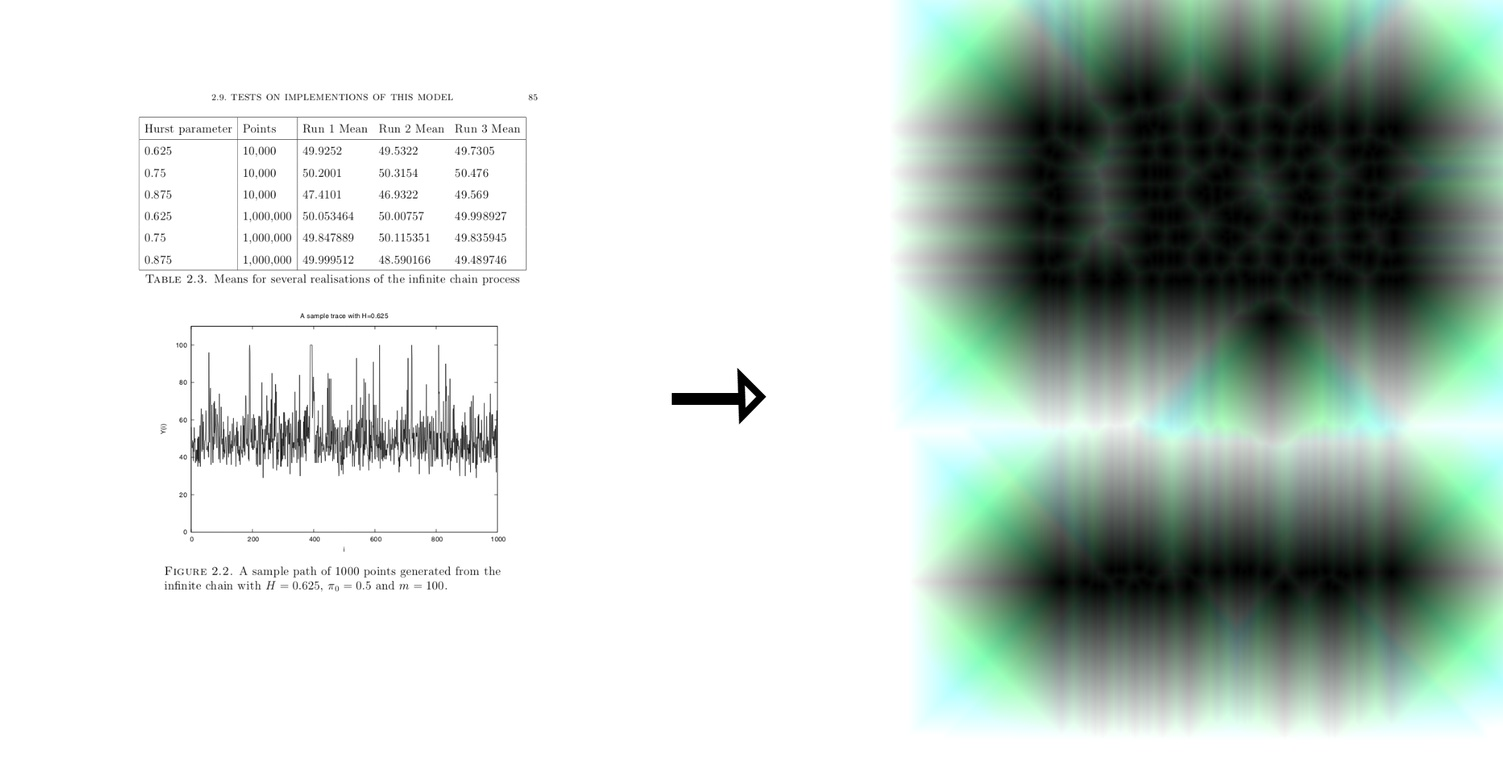
\includegraphics[width=1\columnwidth]{image-transformation} 
        \caption{Esempio di trasformazione dell'immagine con il calcolo delle distanze}
        \label{img:distance-transformation}
    \end{figure}
    Innanzitutto con questa trasformazione si possono annidare più informazioni - relative alle tre trasformazioni - su tre canali. Poi possiamo vedere come l'immagine assomigli di più ad una che la rete neurale pre-allenata si aspetterebbe: ovvero con una distribuzione semi omogenea di pixel, all'interno dei quali cercare le ricorrenze del caso. Possiamo infatti vedere come il grafico sia scarsamente rappresentato, poiché la quantità di pixel "colorati" è mediamente bassa. Lo è di più nella sua descrizione, ad esempio; inoltre intravediamo una certa organizzazione nella trasformazione della tabella: proprio quello che stavamo cercando!
    
    \subsection{Preparazione delle etichette}
    Le etichette del \textit{dataset} sul quale ho lavorato erano sotto forma di XML, uno per ogni immagine, all'interno del quale erano presenti le informazioni riguardandi le \textit{boxes} che racchiudono gli oggetti presenti nelle immagini. Poiché \grayname{Tensorflow} accetta solamente formati \grayname{pandas}\cite{prod:pandas} per le etichette, ho provveduto a trasformare le informazioni in due CSV distinti, uno per il training e l'altro per il test.
    
    \subsection{Creazione dei file \textit{TFRecord}}
    Creare i file \textit{TFRecord}, ovvero dei files di input che \grayname{Tensorflow} possa capire, avendo immagini ed etichette pronte, è abbastanza facile. \'E bastato infatti personalizzare lo script\cite{site:generate-tfrecord} offerto direttamente dall'API di Google.
    
    \subsection{Allenamento della rete neurale personalizzata}
    Come già anticipato è stato possibile non concentrarsi sul codice da scrivere per personalizzare la rete e riuscire a gestirla da un file di configurazione. I parametri - o, altresì chiamati nel gergo, \textit{hyperparameters} -, sono tanti e ognuno ha un'importanza maggiore o minore rispetto agli altri. Inoltre ho avuto la possibilità di scegliere da quale tipologia di architettura di rete neurale partire.
    \medskip
    \\L'allenamento è stato effettuato con la mia macchina, della quale caratteristiche scriverò brevemente:
    \begin{itemize}
        \item \textit{CPU}: Intel Core i5 8300H, 3.80GHz in Turbo Mode;
        \item \textit{GPU}: NVidia GTX1050 GDDR5 4GB RAM;
        \item \textit{RAM}: 8GB DDR4 2667MHz;
        \item \textit{Storage}: SSD NVMe 256GB
    \end{itemize}
        \subsubsection{Scelta della rete di partenza}
        Per quanto riguarda la scelta dei pesi iniziali, ovvero della rete neurale di partenza, non avendo molto tempo a disposizione ho deciso di effettuare una decisione a priori guardando le statistiche\cite{site:COCO-trained-model-statistics} degli allenamenti delle reti basati sul \textit{dataset} COCO\cite{site:coco-dataset}. La rete con risultati migliori a parità di velocità si è rivelata essere la \grayname{faster\textunderscore rcnn\textunderscore inception\textunderscore v2\textunderscore coco}, ho quindi basato tutti i miei successivi esperimenti su questa.
        \subsubsection{Scelta dei parametri da personalizzare}
        Per quanto invece concerne la scelta dei parametri, ho deciso di focalizzare la mia attenzione su alcuni di questi:
        \begin{itemize}
            \item \textit{image\textunderscore resizer}, che si occupa della dimensione e dei protocolli di ridimensionamento delle immagini;
            \item \textit{l2\textunderscore regulizer}, ovvero il peso della trasformazione L2\cite{site:l2-reg};
            \item \textit{first\textunderscore stage\textunderscore nms\textunderscore iou\textunderscore threshold} e \textit{iou\textunderscore threshold}, ovvero il peso dato all'IoU;
            \item \textit{optimizers} e \textit{learning\textunderscore rate}, ovvero la tipologia di \textit{optimizer}\cite{site:type_optimizers} utilizzato e come gestire il \textit{learning rate}.
        \end{itemize}
        Ho scelto di personalizzare solo questi principalmente per via della letteratura e dei corsi che ho seguito: questi infatti consigliavano di concentrarsi su questi parametri innanzitutto, poi di esplorare gli altri. Non avendo a disposizione molto tempo per testare ho quindi pensato di effettuare questa scelta.
        
        \subsubsection{Esempio di utilizzo di \grayname{Tensorboard}}
        \grayname{Tensorboard} è stato un valido alleato nell'allenare le reti neurali. Durante l'apprendimento permette di vedere l'andamento di due curve: una in arancione relativa al \textit{training}, una in blu relativa alla valutazione - che poi è quella più rilevante come "risultato". In particolare, i grafici che più ho tenuto sotto controllo sono stati:
        \begin{itemize}
%            \itemsep0em 
            \item la \textit{DetectionBoxes\textunderscore Precision/mAP (large)}, principalmente perché la maggior parte delle scatole da individuare corrispondevano a dimensioni generose, essendo le tabelle relativamente grandi rispetto all'immagine. Nell'immagine \ref{img:example_tensorboard_1} possiamo vedere la valutazione di una rete con \textit{adam optimizer};
            \item La \textit{loss}, per valutare se il \textit{training} o la valutazione stessero andando in \textit{overfitting}. Nell'immagine \ref{img:example_tensorboard_2} possiamo vedere l'andamento della perdita per una rete neurale con \textit{momentum optimizer}.
        \end{itemize}
        \begin{figure}[!h] 
            \centering
            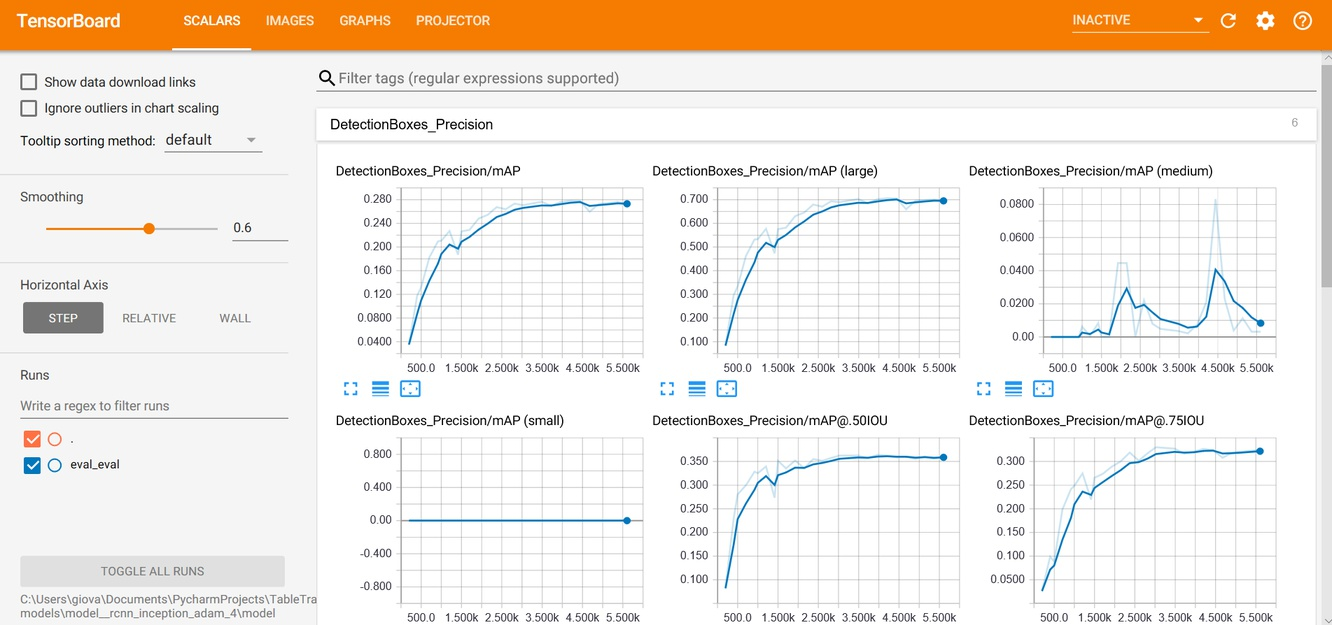
\includegraphics[width=1\columnwidth]{tensorboard-1} 
            \caption{Esempio di schermata classica con Tensorboard}
            \label{img:example_tensorboard_1}
        \end{figure}
        \begin{figure}[!h] 
        \centering
        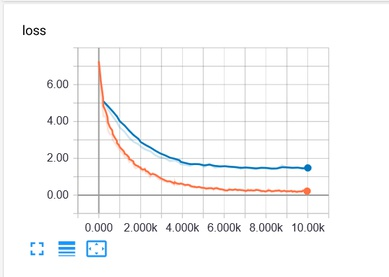
\includegraphics[width=0.7\columnwidth]{tensorboard-2} 
        \caption{Esempio di loss con \textit{Momentum Optimizer}}
        \label{img:example_tensorboard_2}
        \end{figure}
        
        \subsubsection{Considerazioni sui parametri}
        \paragraph{\textit{image\textunderscore resizer}}
        ~\\La personalizzazione di questo parametro è stata piuttosto semplice: ho dovuto trovare un buon compromesso tra grandezza dell'immagine da passare come input e la quantità di memoria a disposizione. Alla fine la scelta di ridimensionare in maniera fissa (quindi non rispettando le proporzioni dell'immagine) ogni immagine come input a $400x400px$ mi ha permesso una buona risoluzione a fronte di un'occupazione decente in RAM. Da notare che non rispettare le proporzioni dell'immagine - ovvero forzare una risoluzione predefinita - mi ha permesso di aumentare la \textit{batch\textunderscore size} oltre il valore predefinito di 1-
        \paragraph{\textit{l2\textunderscore regulizer}}
        ~\\L'impostazione di questo parametro è correlato alla presenza di \textit{overfitting} nel proprio modello. Grazie a \grayname{tensorboard} ho potuto tenere d'occhio l'andamento degli apprendimenti e, dopo molti tentativi, ho capito che probabilmente il valore che più si addice al mio \textit{dataset} è di $1*10^{-4}$ come valore iniziale, che poi aumenta fino a $4*10^{-4}$.
        \paragraph{\textit{first\textunderscore stage\textunderscore nms\textunderscore iou\textunderscore threshold} e \textit{iou\textunderscore threshold}}
        ~\\Questi due parametri gestiscono la metrica dell'IoU. Ho deciso di mettere mano anche a questo parametro dopo aver visionato il comportamento delle reti neurali quando testate (sezione \ref{sec:test-boxes}). Infatti mi sono reso conto che molto spesso la rete neurale confondeva una parte delle tabelle che avrebbe dovuto trovare per la tabella intera. Questo fatto è dovuto probabilmente alla diversità delle immagini del \textit{dataset} utilizzato per il training e di quelle che poi effettivamente sono presenti all'interno delle polizze. Un modo per mitigare questo effetto è stato quindi quello di abbassare il valore di questi due parametri a $0.5$.
        \paragraph{\textit{optimizers} e \textit{learning\textunderscore rate}}
        ~\\La scelta di questi due parametri è stata dettata dalla disponibilità dell'API di Google, dalla presenza di parametri di default e dalla letteratura. In particolare la disponibilità di \textit{optimizers} da parte dell'API è di:
        \begin{itemize}
            \item \textit{RMSPropOptimizer}\cite{site:RMSProp-optimizer};
            \item \textit{MomentumOptimizer}\cite{site:momentum-optimizer};
            \item \textit{AdamOptimizer}\cite{site:adam-optimizer}.
        \end{itemize}
        La scelta predefinita era impostata sul \textit{Momentum}. Tuttavia nei corsi seguiti su Coursera era emerso che l'\textit{Adam} avesse una migliore performance, a patto di regolare correttamente il \textit{learning rate}. Ho eseguito alcune prove con il \textit{momentum}, poi ho deciso di cambiare. Quindi, dopo aver impostato l'\textit{Adam} e il relativo \textit{learning rate} con la seguente formula (dell'\textit{exponentially decay learning rate}), dati $l_{r0}$ \textit{learning rate} iniziale, $t$ il numero di iterazioni e $k$ un parametro:
        \[l_r=l_{r0} * e^{(-k*t)}\]
        e dopo molte prove - per evitare un apprendimento troppo veloce oppure troppo lento -, sono arrivato ad impostare:
        \[l_{r0}=1exp^{-4}\]
        \[k=0.8\]
        \[decay\textunderscore steps=300\]
        dove \textit{decay\textunderscore steps} sono i passi dopo i quali valutare il nuovo \textit{learning rate}.
        
        \subsubsection{Interpretazione e modifica delle \textit{boxes}}
        \label{sec:interpretazione-modifica-boxes}
        La rete neurale è per lo più rimasta in allenamento per 7000 iterazioni per un tempo variabile tra le 4 e le 8 ore di tempo. Una volta esportato il grafo congelato, così da essere pronto per l'inferenza, ho potuto testare le varie configurazioni. In \ref{sec:test-boxes} troviamo i risultati visivi di quelle provate.
        \medskip
        \\Ci si rende subito conto di come l'identificazione delle tabelle non sia precisa. Soprattutto si nota come il più delle volte l'algoritmo confonde una parte per l'insieme, identificando solamente porzioni di tabella e spesso in maniera sovrapposta tra una identificazione e l'altra. Inoltre anche i punteggi non sono mai eccelsi: non appena si supera la valutazione di $0.8$ l'identificazione inizia ad essere lacunosa. 
        \medskip
        \\Ho quindi pensato ad una soluzione. Dal momento che conoscevo la tipologia di documenti che avrei dovuto analizzare, ho stilato le seguenti osservazioni:
        \begin{itemize}
            \item ogni tabella compare sempre senza testo attorno e a singola colonna;
            \item non ci sono mai più di quattro tabelle nella stessa pagina;
            \item le tabelle sono in formato misto, ma per lo più composto di parole e numeri.
        \end{itemize}
        Da queste informazioni ho dedotto di poter:
        \begin{itemize}
            \item tagliare la pagina non attorno alla scatola trovata ma su tutta la larghezza di quella. Così avrei diminuito l'errore dovuto all'individuazione, dovendo considerare solo due punti invece di quattro forniti (posizione di minimo e di massimo sull'asse verticale);
            \item unire le informazioni di alcune scatole con un punteggio abbastanza alto (personalmente impostato a $0.6$) che venivano tra loro sovrapposte, generando quindi un'unica grande \textit{box}.
        \end{itemize}
        Nella sezione \ref{sec:test-boxes} si potranno apprezzare le nuove scatole che, in rosso, individuano quindi la zona che si dovrà andare a tagliare.
    

\newpage
\section{IntelligentOCR}
    \subsection{\textit{Overview generale}}
    \grayname{IntelligentOCR} è l'effettivo programma che la mia azienda può utilizzare in maniera produttiva. Si occupa di distinguere le tabelle all'interno di documenti PDF - nel mio particolare caso, in polizze assicurative -, per poi poter processare in maniera diversa le une e il testo rimanente. Quindi, questo programma:
    \begin{enumerate}
        \item prende come input un file PDF e lo trasforma in immagini;
        \item per ogni immagine, ricerca tabelle al suo interno;
        \item processa ogni tabella con un estrattore di tabelle da documenti, così da restituirne la struttura e da restituirla su CSV;
        \item processa le immagini con testo puro al loro interno per estrarre del testo su TXT.
    \end{enumerate}
    Il focus durante la progettazione di questo programma è stato la leggibilità del codice e la leggerezza in RAM, poiché il programma è destinato a funzionare su un server con relativamente poca memoria a disposizione e ad essere manutenuto e migliorato da altre persone.
    
    \subsection{\textit{Design pattern} utilizzati}
    Tutti i passaggi di cui sopra mi hanno indotto a pensare ad una sorta di "catena di montaggio" per il mio prodotto, che lo rendesse facilmente migliorabile e testabile. Questo soprattutto in un'ottica aziendale: difficilmente mi occuperò di manutenere il prodotto che ho creato e un'altra persona dovrà riuscire a manutenerlo senza fatica.
    \medskip
    \\Essendo una sequenza di azioni non correlate fra loro ho pensato che il \textit{Pipeline Pattern}\cite{site:pipeline-pattern} potesse venirmi in aiuto. Infatti questo garantisce un'ottimo approccio per testare e per applicare il \textit{single responsibility principle}\cite{site:single-responsibility-principle}, in quanto ogni pezzo di codice fa solamente la sola o le due uniche cose per le quali è stato progettato, dopodiché passa il testimone al pezzo successivo. Non da meno, aumenta in maniera esponenziale la leggibilità del programma.
    \medskip
    \\Non da ultimo è da notare che è stato eseguito un approccio \textit{bottom-up}, ovvero dal basso verso l'alto. Ho cercato di costruire prima tutti i passaggi in maniera autonoma, senza che gli uni dipendessero dagli altri; ho poi provveduto alla composizione dei vari pezzi. Si può notare questo approccio nella composizione del file \textit{pipeline.py}, dove non vengono effettuate operazioni aggiuntive ma vengono solamente invocati i vari anelli della catena.
    
    \subsection{La \textit{pipeline}}
    Poiché il prodotto si configura proprio come una \textit{pipeline}, ne mostrerò la progettazione per parti. Si può apprezzare il fatto che ogni step è separato dagli altri in maniera stagna, tant'è che si può attivare l'output su disco oppure testare con documenti o immagini di prova in qualunque punto della catena di montaggio. 
        \subsubsection{Da PDF ad immagini}
        Un PDF è di per sé un formato prestante: può anche contenere delle informazioni relative al layout che poi possono essere utilizzate da lettori più o meno avanzati. Per questo motivo se un PDF non è frutto di una scansione, ma anzi è stato "stampato" digitalmente, allora tutto ciò che riguarda l'inferenza con rete neurali, la suddivisione in tabelle e testo, non ha più senso d'esistere perché esistono già molti strumenti che si occupano di interpretare tabelle.
        Tuttavia l'azienda mi ha esplicitamente chiesto di coprire il caso generale, ovvero di PDF provenienti da scansioni. In effetti si è poi capito che la stragrande maggioranza delle polizze assicurative presenti nel database era composto da PDF di siffatta natura.
            \paragraph{Estrazione}
            Ho quindi inizialmente provveduto all'utilizzo di \grayname{Wand}\cite{prod:wand}, \textit{wrapper} attorno a \grayname{ImageMagik}\cite{prod:imagemagik}, che esportava tutte le immagini in memoria, per poi poterle utilizzare nel resto della catena di montaggio. Tuttavia, dopo aver testato in maniera più approfondita il prodotto, mi sono reso conto che la memoria veniva occupata per centinaia di MB inutilmente, in quanto venivano caricate tutte le immagini del documento per poi comunque processarne una alla volta. Inoltre \grayname{ImageMagik} è affetto da un bug che, in caso di PDF di grandi dimensioni, fa sì che non liberi lo spazio temporaneo occupato su hard disk, portando all'occupazione di decine di GB inutilmente. Tutto ciò mi ha portato a cambiare approccio: innanzitutto ho proceduto all'utilizzo di \grayname{pdftoppm}\cite{prod:pdftoppm} da riga di comando direttamente da Python. Questo mi ha permesso di accedere una pagina alla volta ad ogni PDF, quindi di avere un'occupazione in RAM minima. Inoltre mi sono informato circa l'utilizzo dei \gls{generators} di Python, regolando quindi l'accesso ad ogni pagina solo quando effettivamente necessario.
            \medskip
            \\Da questo punto in poi tutti i passaggi vengono eseguiti su una pagina alla volta.
            \paragraph{Miglioramento dell'input}
            Una volta ottenuta la pagina possono essere eseguiti dei miglioramenti sull'input. In questo progetto viene solamente applicato un raddrizzamento attraverso \grayname{Alyn}\cite{prod:alyn}, ma è in questa sede che è possibile applicare altre trasformazioni. Una possibilità studiata ma non applicata in quanto non richiesto e per mancanza di tempo sarebbe stata la riduzione del rumore di fondo ispirandosi a dei \textit{kernels}\cite{site:denoysing-dirty-documents} offerti da Kaggle\cite{site:kaggle}.
        \subsubsection{Da immagini a ritagli}
        In questo stadio viene eseguita l'inferenza con la rete neurale descritta nella sezione \ref{sec:interpretazione-modifica-boxes}. Qui vengono replicati gli stessi passi: viene convertita l'immagine in un formato più "gradevole" per la rete neurale, vengono emesse le \textit{boxes} e vengono interpretate. A questo punto viene eseguito il taglio vero e proprio: si crea quindi una lista di immagini, in ognuna delle quali vengono memorizzate tutte le tabelle ritagliate dalla pagina originale, e un'immagine unica in cui vengono uniti tutti i ritagli rimanenti.
        \medskip
        \\A questo punto la lista di immagini e quella singola con tutto il testo vengono processate in maniera diversa.
        \subsubsection{Da tabelle a CSV}
        Ogni tabella della lista viene convertita ciascuna in un file PDF ricercabile con \grayname{Tesseract}\cite{prod:tesseract}. Questo è infatti l'unico formato che \grayname{Tabula}\cite{prod:tabula} accetta come input, per poter poi esportare la struttura calcolata.
        \subsubsection{Da immagini a testo puro}
        Ogni collage di immagini rimanenti dopo l'estrazione delle tabelle viene invece processato semplicemente da \grayname{Tesseract} e viene prodotto un file TXT con all'interno tutto il testo che lo strumento è riuscito a comprendere.
    \subsection{Risultati ottenuti}
    I risultati si possono visionare alla sezione \ref{sec:crop-polizze-assicurative}. Si può notare come non siano ancora ottimali. Come si può osservare alla sezione \ref{sec:good-test} nel caso di documenti ben formati il riconoscimento è sufficiente; tuttavia, se i documenti sono scansionati male, l'algoritmo funziona molto peggio (ad esempio in sezione \ref{sec:bad-test}). \'E tuttavia un passo in avanti notevole nella distinzione tra i due tipi di contenuti, sui quali poi si potranno eseguire altri tipi di analisi.
    
    
    
    
    
